% Created 2025-02-09 dom 16:38
% Intended LaTeX compiler: lualatex
\documentclass[presentation,professionalfonts,aspectratio=169]{beamer}
                

% 
\makeatletter
 \@ifclassloaded{beamer}{%
  %%% save beamer's `solution' environment as `beamersolution':
  \let\beamersolution\solution
  \let\endbeamersolution\endsolution
  %%% "delete" the `solution' environment:
  \let\solution\relax
  \let\endsolution\relax
}{%
}%
\makeatother
\usepackage[utf8]{inputenc}
\usepackage[T1]{fontenc}
%\usepackage[french]{babel}
\usepackage[portuguese]{babel}

%%%% FONTS




\usepackage{xsim}
\usepackage[most]{tcolorbox}
\usepackage{amssymb}
\usepackage{fontawesome}
\newcounter{paragraph}



\DeclareExerciseEnvironmentTemplate{custom}{%
  \begin{tcolorbox}[boxrule = 0pt]
  \tcbox[on line,colback=teal,colframe=teal,coltext=white,size=small]{%
    \faBook\sffamily\bfseries\
    \XSIMmixedcase{\GetExerciseName}
    \GetExerciseProperty{counter}%
  }\quad
}{\end{tcolorbox}}


\DeclareExerciseEnvironmentTemplate{custom2}{%
  \begin{tcolorbox}[boxrule = 0pt]
  \tcbox[on line,colback=violet,colframe=violet,coltext=white,size=small]{%
    \faToggleOn\sffamily\bfseries\
    \XSIMmixedcase{\GetExerciseName}
    \GetExerciseProperty{counter}%
  }\quad
}{\end{tcolorbox}}




\DeclareExerciseType{test}{
	exercise-env = question ,
	solution-env = answer ,
	exercise-template = custom ,
	solution-template = custom2 ,
	exercise-name	= Exemplo. ,
	exercises-name = Exemplo ,
	solution-name = Solução ,
	solutions-name = Sol. ,
	exercise-heading = \textbf ,
	solution-heading = \textbf
}


\xsimsetup{
  exercise/within = section,
  exercise/the-counter =  \arabic{exercise}, 
%%solution-name = solution,  % used with headings=true
solution/print=false,
%print-collection/print=both,
}





\usepackage{colortbl}
\usepackage[tikz]{bclogo}
\usetikzlibrary{fit,patterns,shadows.blur,shapes,mindmap}
\usetikzlibrary{arrows,calc,arrows.meta,decorations.markings,shapes.symbols}
\usetikzlibrary{decorations.pathreplacing, decorations.pathmorphing,calc,arrows,positioning}
\usepackage{tikzpeople}
\usepackage{qrcode,hyperref}
\usepackage{upgreek}
%\usepackage[version=4]{mhchem}
\usepackage{tabularray}


\NewTblrTheme{fancy}{
\SetTblrStyle{caption-tag}{font=\bfseries}
\SetTblrInner[tblr,longtblr]{rowsep=2.5pt}
\DefTblrTemplate{firsthead, middlehead,lasthead}{default}{} % <---
\DefTblrTemplate{contfoot-text}{normal}{\scriptsize\textit{Continued on the next page}}
\SetTblrTemplate{contfoot-text}{normal}
}






\usepackage{chemfig,chemmacros,elements,chemformula}
\chemsetup{modules={all}}
\chemsetup[redox]{pos=top,roman=false}
\chemsetup[redox]{pos=top}
\chemsetup{redox/sep=.5em}
\chemsetup[redox]{explicit-sign=true}
\NewChemPhase\lqdd{\(\ell\)}
\NewChemPhase\gr{grafite}
\NewChemPhase\reac{reação}
\NewChemState\Enthalpy{symbol=H,superscript=,unit=\kilo\joule}%
\usepackage{siunitx}
\setchemfig{fixed length=false, atom sep=2.5em, arrow offset=6pt, scheme debug=false}%,angle increment=30}
\renewcommand*\printatom[1]{\ensuremath{\mathsf{#1}}} % This line changes the font of the atoms to sans serif
%%%% QRCODE
\usepackage{pdfpages}
\usepackage{mol2chemfig}
\usepackage{subfig,caption}
\usepackage{wrapfig}
\usepackage{enumitem}
\setitemize{label=\usebeamerfont*{itemize item}%
\usebeamercolor[fg]{itemize item}
\usebeamertemplate {itemize item}}
\usepackage{array} % ajust colunm table
\usepackage{cancel}
\usepackage[controls]{animate}
\renewcommand{\CancelColor}{\color{red}}

%%%%%%%%%%%%%%%%%%% CONFIG TCOLORBOX 

\newtcolorbox{mybox}[2][]{boxsep=0.5em,left=0.5em,
colback=blue!5!white, colframe=blue!75!black,
fonttitle=\bfseries\sffamily,
colbacktitle=blue!85!red!60,enhanced,
attach boxed title to top left={yshift=-3mm,xshift=5mm},
title=#2,#1}

\newtcolorbox{myrule}[2][]{boxsep=0.5em,left=0.5em,
colback=green!5!white, colframe=blue!75!black,
fonttitle=\bfseries\sffamily,
colbacktitle=blue!85!red!60,enhanced,
attach boxed title to top left={yshift=-3mm,xshift=5mm},
title=#2,#1}


\newtcolorbox{myex}[2][]{boxsep=0.5em,left=0.5em,
  colback=yellow!5!white, colframe=blue!75!black, 
  fonttitle=\bfseries\sffamily,
  colbacktitle=blue!85!red!60,enhanced,
  attach boxed title to top left={yshift=-3mm,xshift=5mm},
  title=#2,#1}


 \definecolor{col1}{HTML}{FF7878}
 \definecolor{col2}{HTML}{51B5F8}
 \definecolor{col3}{HTML}{68E1AA}
 \definecolor{col4}{HTML}{B869EA}
 \definecolor{col5}{HTML}{FF5500}
 \definecolor{col6}{HTML}{FFF8E7}
 \definecolor{col7}{HTML}{FF9966}
 \definecolor{col8}{HTML}{9400D3}



\definesubmol\nobond{-[,0.2,,,draw=none]\scriptstyle\color{blue}}
\newcommand{\re}{\hspace{-1cm}}
\newcommand{\af}{\hspace{2cm}}

%%%% Config X sim for BEAMER
\usepackage{ragged2e}
\justifying
\makeatletter
\@ifclassloaded{beamer}{%
%%% save beamer's `solution' environment as `beamersolution':
\let\beamersolution\solution
\let\endbeamersolution\endsolution
%%% "delete" the `solution' environment:
\let\solution\relax
\let\endsolution\relax
}{%
}%
\makeatother
\usepackage[utf8]{inputenc}
\usepackage[T1]{fontenc}
%\usepackage[portuguese, ]{babel}
%\usepackage[br]{pgf-PeriodicTable}
%%%% FONTS
%%% XSIM CONFIG BEAMER
\usepackage{xsim}
\usepackage{amsmath}
\usepackage[most]{tcolorbox}
\usepackage{amssymb}
\usepackage{fontawesome}
\usepackage{tasks}
\newcounter{paragraph}
%\usepackage[dvipsnames,svgnames]{xcolor}
\usepackage[dvipsnames]{xcolor}
%\usepackage{annotate-equations}
%%% BOX EXERCISE BEAMER
\DeclareExerciseEnvironmentTemplate{custom}{%
\begin{tcolorbox}[boxrule = 0pt]
\tcbox[on line,colback=teal,colframe=teal,coltext=white,size=small]{%
\faBook\sffamily\bfseries\
\XSIMmixedcase{\GetExerciseName}
\GetExerciseProperty{counter}%
}\quad
}{\end{tcolorbox}}
%% == CUSTOM BOX BEAMER
\DeclareExerciseEnvironmentTemplate{custom2}{%
\begin{tcolorbox}[boxrule = 0pt]
\tcbox[on line,colback=violet,colframe=violet,coltext=white,size=small]{%
\faToggleOn\sffamily\bfseries\
\XSIMmixedcase{\GetExerciseName}
\GetExerciseProperty{counter}%
}\quad
}{\end{tcolorbox}}
\DeclareExerciseType{test}{
exercise-env = question ,
solution-env = answer ,
exercise-template = custom ,
solution-template = custom2 ,
exercise-name = Exemplo ,
exercises-name = Exemplo ,
solution-name = Solução ,
solutions-name = Sol. ,
exercise-heading = \textbf ,
solution-heading = \textbf
}
\xsimsetup{
exercise/within = section,
exercise/the-counter =  \arabic{exercise},
%%solution-name = solution,  % used with headings=true
solution/print=true,
print-collection/print=both,
}
\NewTasksEnvironment[label = (\emph{\alph*}),
label-width = 12pt]{choice}[\choice]
\usepackage{empheq} %%% Brackers
\usepackage{colortbl}
\usepackage[tikz]{bclogo}
\usetikzlibrary{calc,fadings,shadings}
\usetikzlibrary{fit,patterns,shadows.blur,shapes,mindmap}
\usetikzlibrary{arrows,snakes,shapes,arrows.meta,decorations.markings,shapes.symbols}
\usetikzlibrary{backgrounds,shapes.geometric}
\usetikzlibrary{decorations.pathreplacing, decorations.pathmorphing,arrows,positioning}
\usepackage{tikzpeople}
\usepackage{qrcode,hyperref}
\usepackage{upgreek}
%\usepackage[version=4]{mhchem}
\usepackage{tabularray}
%%% PACKAGE PLOT GRAPH
\usepackage{pgfplots}
\pgfplotsset{width=10cm,compat=1.9}
%%% CUSTOM TABLE
\NewTblrTheme{fancy}{
\SetTblrStyle{caption-tag}{font=\bfseries,red2}
\SetTblrInner[tblr,longtblr]{rowsep=2.5pt}
\DefTblrTemplate{firsthead, middlehead,lasthead}{default}{} % <---
\DefTblrTemplate{contfoot-text}{normal}{\scriptsize\textit{Continua ...}}
\SetTblrTemplate{contfoot-text}{normal}
}
%% ==== CHEMMACROS E CHEMFIG CONFIG
\usepackage{chemfig,chemmacros,elements,chemformula}
\chemsetup{modules={all}}
\chemsetup[redox]{pos=top,roman=false}
\chemsetup[redox]{pos=top}
\chemsetup{redox/sep=.5em}
\chemsetup[redox]{explicit-sign=true} %%% reaction redox
%% == CUSTOM PHASES IN CHEMMACROS
\NewChemPhase\lqdd{\(\ell\)}
\NewChemPhase\gr{grafite}
\NewChemPhase\reac{reação}
\NewChemState\Enthalpy{symbol=H,superscript=,unit=\kilo\joule\per\mole}%
\NewChemState\Entalpia{symbol=H,superscript=,unit=\kilo\cal\per\mole}%
\usepackage{siunitx}
\setchemfig{fixed length=false, atom sep=2.5em, arrow offset=6pt, scheme debug=false}
%% == NUMEROS PARA FORMULES
\renewcommand*\printatom[1]{\ensuremath{\mathsf{#1}}} % This line changes the font of the atoms to sans serif
%%% INCLUDE PAGES PDFs
\usepackage{pdfpages}
\usepackage{mol2chemfig}
\usepackage{xymtexpdf}
%\changeunitlength{0.08pt}
%%\wedgehasheddash
\usepackage{subfig,caption}
\usepackage{wrapfig}
\usepackage{enumitem}
\setitemize{label=\usebeamerfont*{itemize item}%
\usebeamercolor[fg]{itemize item}
\usebeamertemplate {itemize item}}
\usepackage{array} % ajust colunm table
\usepackage{cancel}
\usepackage[controls]{animate}
%\usepackage{movie15}
\renewcommand{\CancelColor}{\color{red}}
%%%%%%%%%%%%%%%%%%% CONFIG TCOLORBOX
\newtcolorbox{mybox}[2][]{boxsep=0.5em,left=0.5em,
colback=blue!5!white, colframe=blue!75!black,
fonttitle=\bfseries\sffamily,
colbacktitle=blue!85!red!60,enhanced,
attach boxed title to top left={yshift=-3mm,xshift=5mm},
title=#2,#1}
\newtcolorbox{myrule}[2][]{boxsep=0.5em,left=0.5em,
colback=green!5!white, colframe=blue!75!black,
fonttitle=\bfseries\sffamily,
colbacktitle=blue!85!red!60,enhanced,
attach boxed title to top left={yshift=-3mm,xshift=5mm},
title=#2,#1}
\newtcolorbox{myex}[2][]{boxsep=0.5em,left=0.5em,
colback=yellow!5!white, colframe=blue!75!black,
fonttitle=\bfseries\sffamily,
colbacktitle=blue!85!red!60,enhanced,
attach boxed title to top left={yshift=-3mm,xshift=5mm},
title=#2,#1}
\tcbset{colback=yellow!10!white, colframe=red!50!black, highlight math style= {enhanced, %<-- needed for the ’remember’ options
colframe=red,colback=red!10!white,boxsep=0pt}}
\definecolor{col1}{HTML}{FF7878}
\definecolor{col2}{HTML}{51B5F8}
\definecolor{col3}{HTML}{68E1AA}
\definecolor{col4}{HTML}{B869EA}
\definecolor{col5}{HTML}{FF5500}
\definecolor{col6}{HTML}{FFF8E7}
\definecolor{col7}{HTML}{FF9966}
\definecolor{col8}{HTML}{9400D3}
%% CONFIG COLOR CARBONO
\tikzstyle{bal}=[inner sep=0.3pt,fill=orange,fill opacity=0.5,circle,minimum size=0.2cm]
\tikzstyle{rect}=[inner sep=0.3pt,fill=red,fill opacity=0.5,circle,minimum size=0.2cm]
\tikzstyle{bal2}=[inner sep=0.3pt,fill=blue,fill opacity=0.5,circle,minimum size=0.2cm]
\tikzstyle{bal3}=[inner sep=0.3pt,fill=yellow,fill opacity=0.5,circle,minimum size=0.2cm]
\definesubmol\nobond{-[,0.2,,,draw=none]\scriptstyle\color{blue}}
\newcommand{\re}{\hspace{-1cm}}
\newcommand{\af}{\hspace{2cm}}
\tikzstyle{mybox} = [draw=red, fill=blue!20, very thick, rectangle, rounded corners, inner sep=10pt, inner ysep=20pt]
\tikzstyle{fancytitle} =[fill=red, text=white]
\date{}
%\usetheme{minflat}
\usetheme{minflat}
\author{Fábio Lima}
\date{}
\title{ Termoquímica}
\hypersetup{
 pdfauthor={Fábio Lima},
 pdftitle={ Termoquímica},
 pdfkeywords={},
 pdfsubject={},
 pdfcreator={Emacs 29.4 (Org mode 9.6.15)}, 
 pdflang={En Portuguese}}
\begin{document}

\begingroup
  \setbeamertemplate{headline}{}
  \maketitle
  \endgroup
\begin{frame}{Sumário}
\tableofcontents
\end{frame}



\section{Termoquímica}
\label{sec:org0db623a}

\begin{frame}[label={sec:org048b2d0}]{Termoquímica}
\begin{description}
\item[{Termoquímica:}] é a parte da Físico-Química voltada para o estudo dos processos que envolvem troca de energia (liberada ou absorvida), sob a forma de \alert{calor}, à pressão constante
\item[{Calor:}] é energia térmica que passa de um corpo em maior temperatura para um corpo de menor temperatura!
\end{description}
\end{frame}



\begin{frame}[label={sec:org2a59a77}]{Entalpia (H)}
\alert{Entalpia (H)} é, de forma simplificada, a quantidade total de energia que se encontra nas substâncias e que pode estar em trânsito, mediante transformações físicas ou químicas.


 \begin{tcolorbox}[ams align*]
 \underbrace{\ch{CH4\gas{} + O2\gas{} }}_{Reagentes}  \ch{->} &      \underbrace{\ch{CO2\gas{} + 2 H2O\lqdd{}}}_{Produtos} \\
 %(Reagentes)     & \; \;         (Produtos)
\end{tcolorbox}

\begin{itemize}
\item A variação de entalpia é dada por:

\begin{tcolorbox}[ams align*]
\Delta H = H_{final}- H_{inicial} \\
\Delta H = H_{produtos} - H_{reagentes}
\end{tcolorbox}
\end{itemize}
\end{frame}






\section{Transformações Químicas}
\label{sec:orgdb09254}

\begin{frame}[label={sec:org7cf1714}]{Processos Endotérmicos}
\begin{itemize}
\item Nas reações endotérmicas, ocorre \alert{absorção} de calor (o sistema \alert{esfria}), a entalpia dos produtos (\(\mathrm{H_p}\)) é \alert{maior} do que a entalpia dos reagentes (\(\mathrm{H_r}\)) e o  \alert{\(\Delta\)H = ( + )}.
\end{itemize}


\begin{bclogo}[logo=\bcinfo]{Exemplo}
%A combustão do álcool etílico \ch{C2H6O_{\lqdd}}
\begin{reactions*}\small
CaCO3_{\sld} -> CaO_{\sld} + CO2_{\gas} & $\qquad \Enthalpy{177.5}$
\end{reactions*}
\end{bclogo}
\end{frame}


\begin{frame}[label={sec:org1931cb4}]{Processos Endotérmicos}
\begin{columns}
\begin{column}{0.45\columnwidth}
\begin{tikzpicture}[scale=1]
	%% 
	% horizontal axis
	\draw[->] (0,0) -- (6,0) node[anchor=north] {Caminho da reação};
	% labels
	% vertical axis
	\draw[->] (0,0) -- (0,5) node[anchor=east] {Entalpia (H)};
	% nominal speed
	\draw[thick,dashed] (0,3) -- (3,3);
	\draw[thick,dashed] (2,1) -- (5.5,1);
	% Us
	\draw[thick] (0,1) -- (2,1) -- (3,3)--(5.5,3);
	\draw (-.47,1) node {$\mathrm{H_{reag.}}$};
	\draw (-.47,3) node {$\mathrm{H_{prod.}}$};
	% Psis
%	\draw[thick] (0,3) -- (2,3) -- (3,1)--(5.5,1);
	\draw[blue] (0.95,1.3) node {\ch{CaCO3\sld}}; %label
	\draw[blue] (4,3.3) node {\ch{CaO\sld{} +  CO2\gas{}}}; %label
	\draw[->,red] (4,1)--(4,3);
	\draw[red](4.6,2) node {$\Delta$H > 0};
	%\draw[blue](3,4.5) node {\ch{aA + bB  ->cC + dD} $\Delta$H > 0};	
\end{tikzpicture}
\end{column}


\begin{column}{0.45\columnwidth}
\begin{center}
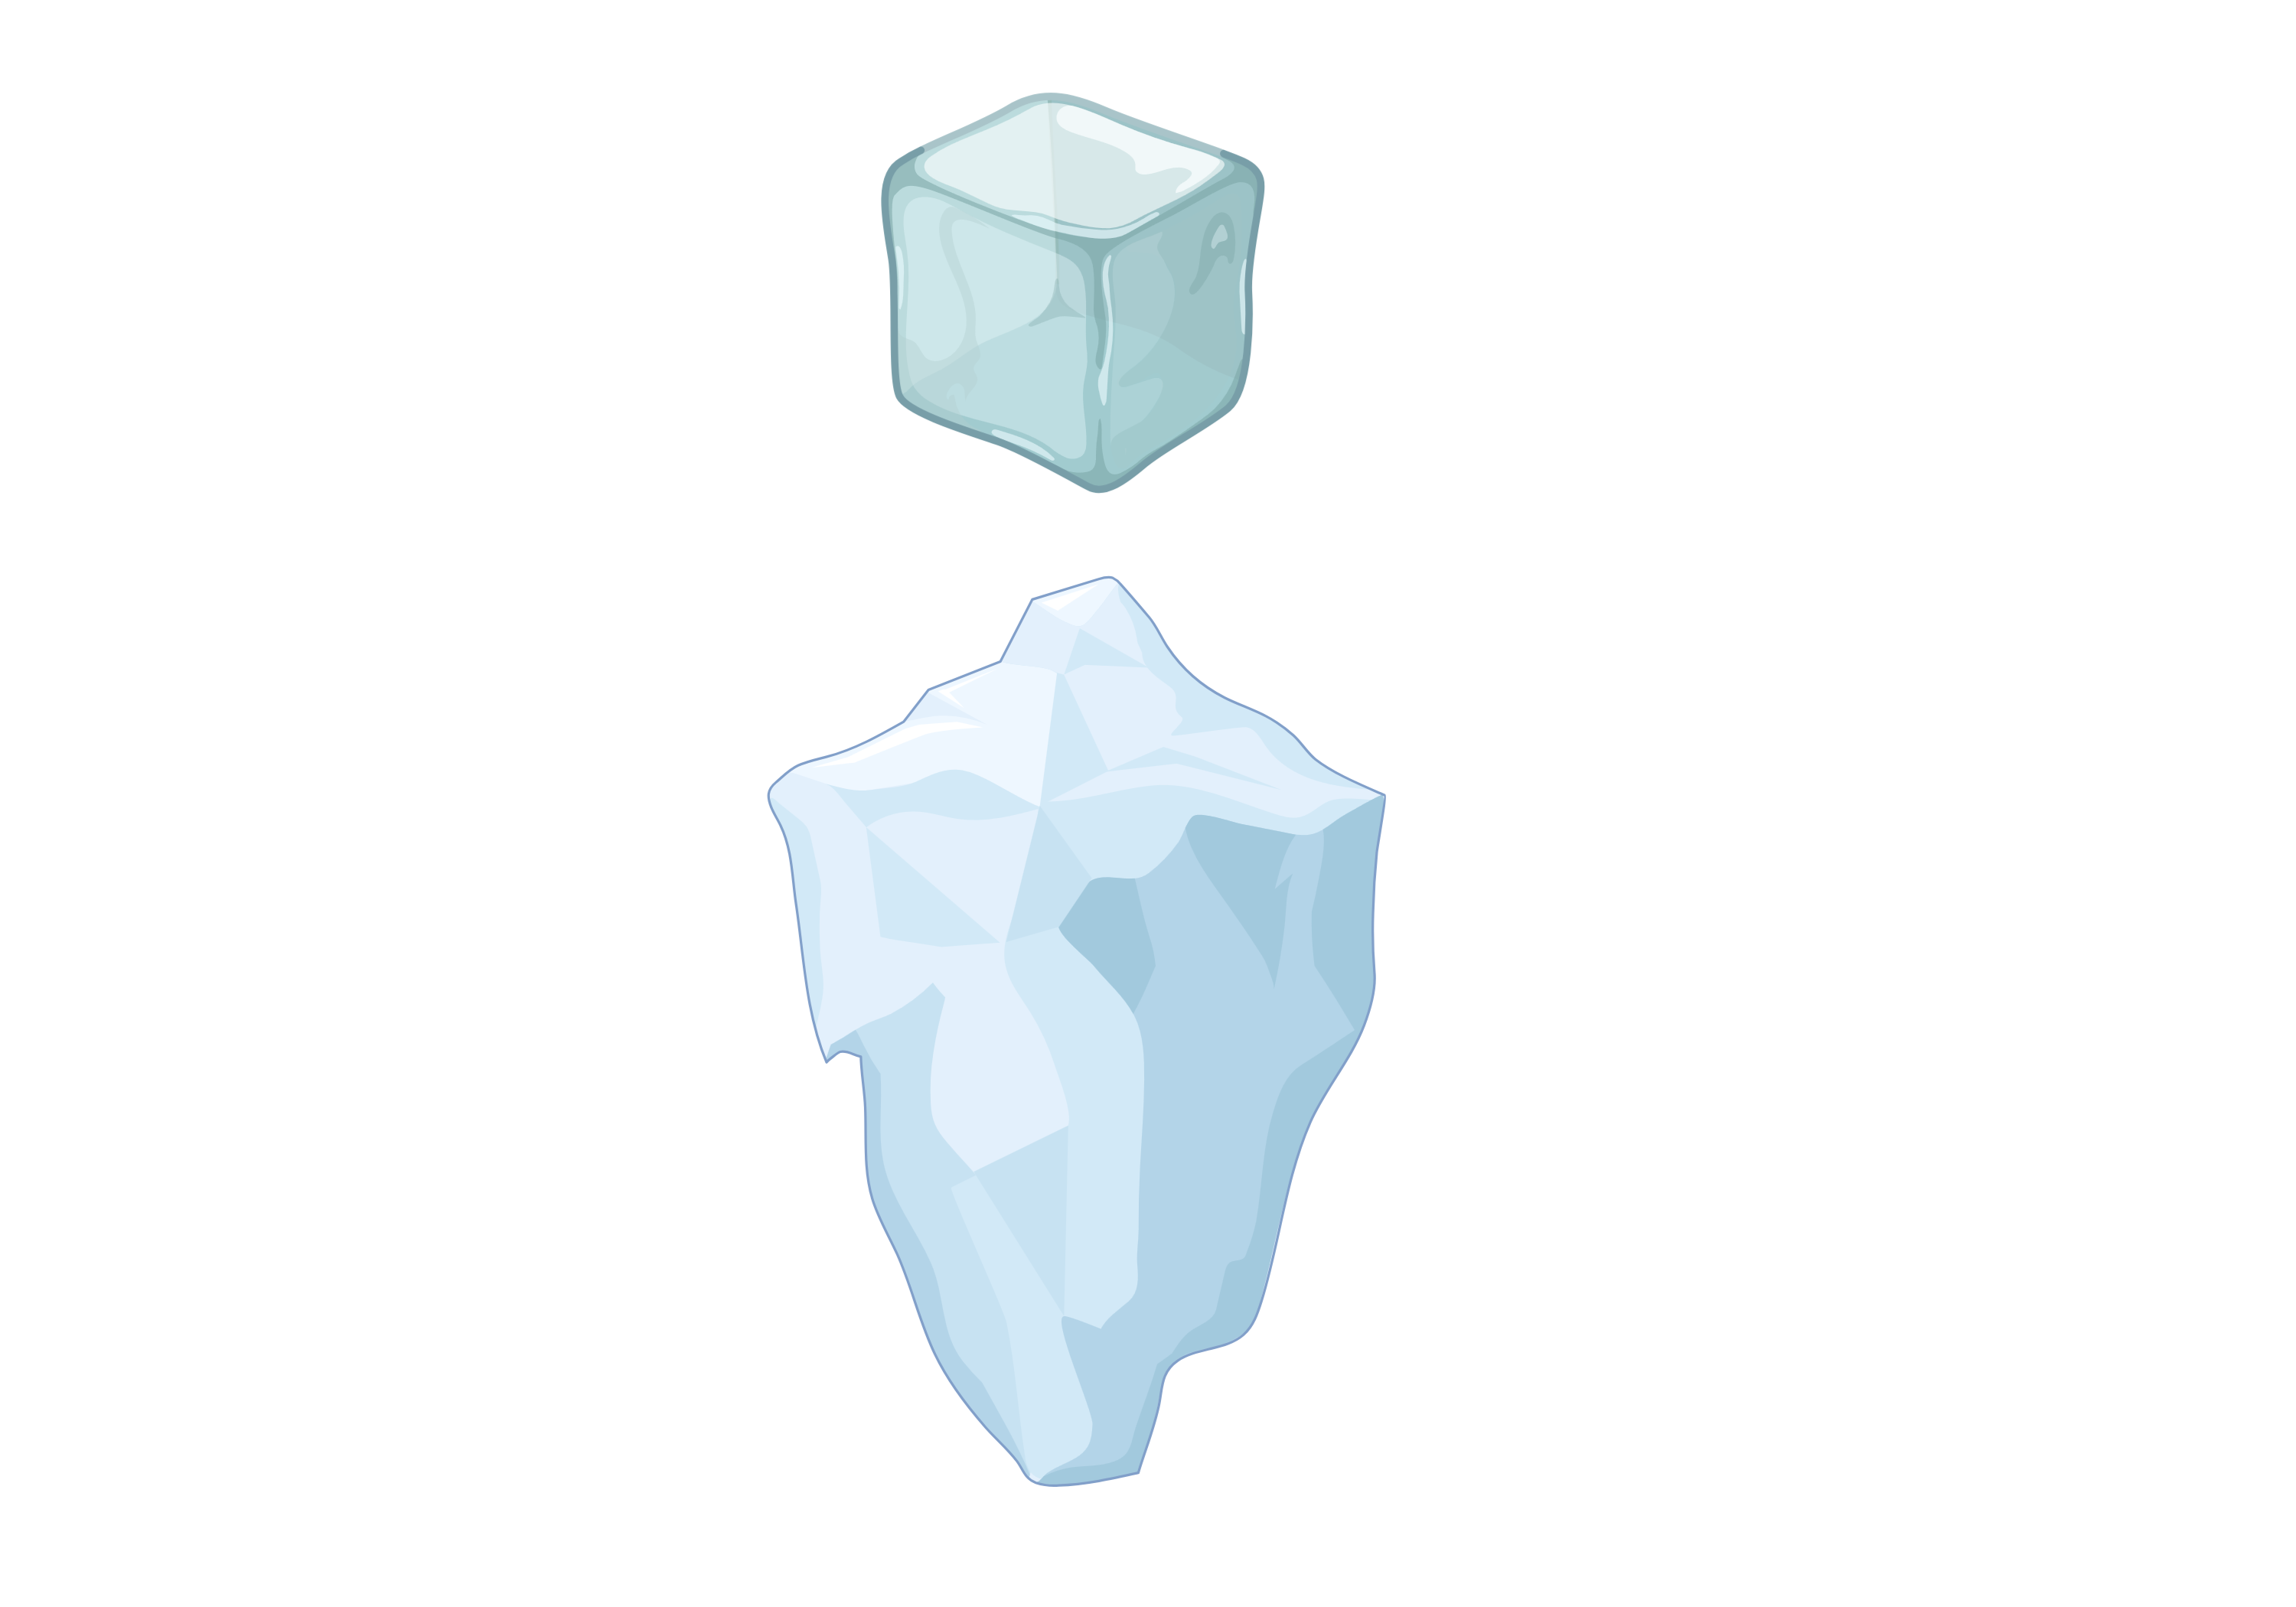
\includegraphics[width=.9\linewidth]{FQ/Termoquimica/gelo.png}
\end{center}
\end{column}
\end{columns}
\end{frame}



\begin{frame}[label={sec:org8cf5168}]{Processos Exotérmicos}
\begin{itemize}
\item Reações exotérmicas, ocorre liberação de calor (o sistema esquenta), a entalpia dos produtos (\(\mathrm{H_P}\)) é menor do que a entalpia dos reagentes (\(\mathrm{H_R}\)) e o  \alert{\(\Delta\)H=(–)}.
\end{itemize}


\begin{bclogo}[couleur=blue!30 , arrondi=0.1 , logo=\bcinfo , epBarre=3.5]{Exemplo}
%A combustão do álcool etílico \ch{C2H6O_{\lqdd}}
\begin{reactions*}\small
C2H6O_{\lqdd} + 3 O2_{\gas} -> 2 CO2_{\gas} + 3 H2O_{\lqdd} & $\qquad \enthalpy[unit=\kilo\joule\per\mole]{-1368}$ \\
%\; \; \;  \(\Delta\)H = – 1368 kJ/mol
\end{reactions*}
\end{bclogo}
\end{frame}


\begin{frame}[label={sec:org5542153}]{Processos Exotérmicos}
\begin{columns}
\begin{column}{0.45\columnwidth}
\begin{tikzpicture}[scale=1]
		%% 
		% horizontal axis
		\draw[->] (0,0) -- (6,0) node[anchor=north] {Caminho da reação};
		% labels
		% vertical axis
		\draw[->] (0,0) -- (0,5) node[anchor=east] {Entalpia (H)};
		% nominal speed
		\draw[thick,dashed] (2,3) -- (5.5,3);
		\draw[thick,dashed] (0,1) -- (3,1);
		% Us
		%\draw[thick] (0,1) -- (2,1) -- (3,3)--(5.5,3);
		\draw (-.45,1) node {$\mathrm{H_{prod.}}$};
		\draw (-.45,3) node {$\mathrm{H_{reag.}}$};
		% Psis
		\draw[thick] (0,3) -- (2,3) -- (3,1)--(5.5,1);
		\draw[blue,font=\small] (1.25,3.3) node {\ch{C2H6O_\lqdd{} + O2_\gas{} }}; %label
		\draw[blue,font=\small] (4.5,1.3) node {\ch{CO2_\gas{} + H2O_\gas{} }}; %label
		\draw[->,red] (1.7,3)--(1.7,1); 
		\draw[red](0.9,2) node {$\Delta$H < 0}; 
		%\draw[blue](3,4.5) node {\ch{aA + bB ->cC + dD} $\Delta$H < 0};	
\end{tikzpicture}
\end{column}


\begin{column}{0.45\columnwidth}
\begin{center}
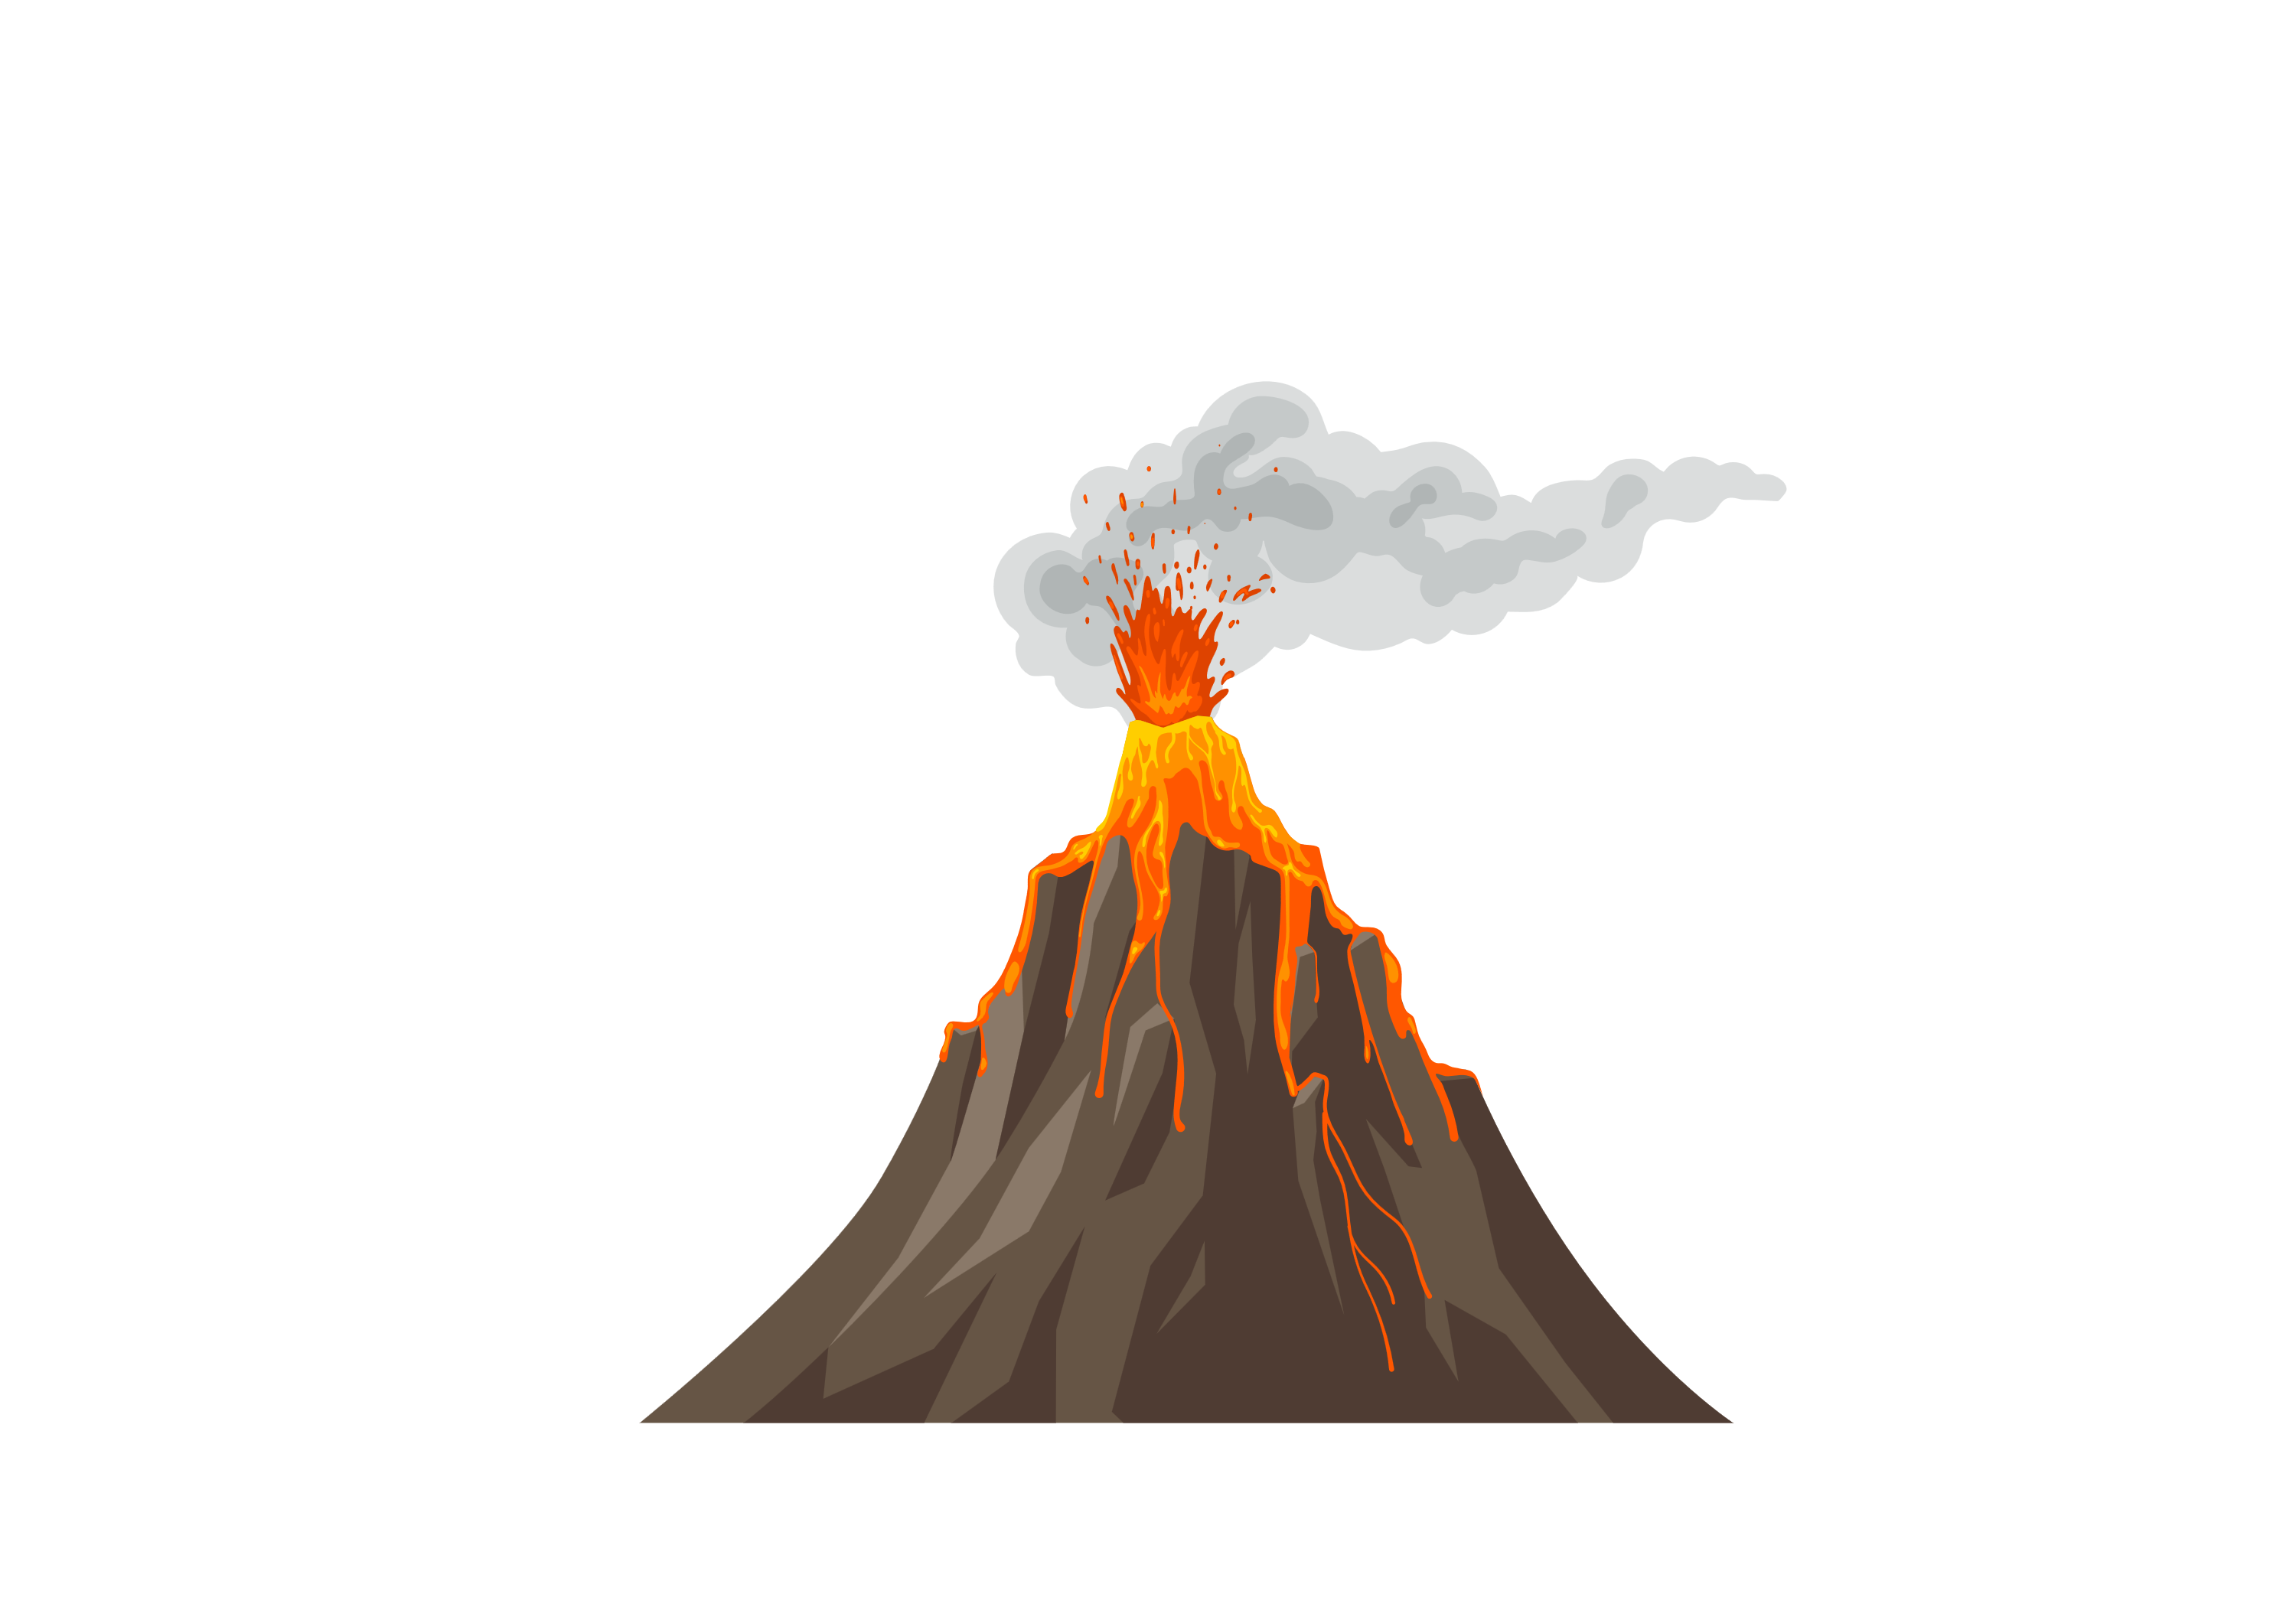
\includegraphics[width=.9\linewidth]{FQ/Termoquimica/vulcao.png}
\end{center}
\end{column}
\end{columns}
\end{frame}



\section{Fatores que influenciam a entalpia}
\label{sec:org898211a}

\begin{frame}[label={sec:org20fd371}]{Fatores que influenciam a entalpia}
\begin{bclogo}[logo=\bcplume]{Principais Fatores}
\begin{itemize}
\item Temperatura
\item Pressão
\item Estado físico
\item Quantidade de matéria
\item Estado alotrópico
\end{itemize}
\end{bclogo}
\end{frame}





\section{Estado Alotrópico}
\label{sec:orgd1eb78b}

\begin{frame}[label={sec:orgf8a19a2}]{Carbono (C)}

\begin{tikzpicture}
% Axis y
\draw[->,ultra thick] (0,0)--(0,5) node[above]{$\Delta$H};
% Axis X
\draw[-,ultra thick] (0,1)--(5,1) node[xshift=-2.3cm,anchor=south] (n1) {Grafite};
 \draw[-,ultra thick] (0,4)--(5,4) node[xshift=-2.3cm,anchor=south] (n2) {Diamante};
\draw[->,ultra thick] (4,1)--(4,3.8);
  \node[blue,font=\bfseries] (c) at (2,2.5) {$\enthalpy{1.9}$};
\node (d) at (7,4) {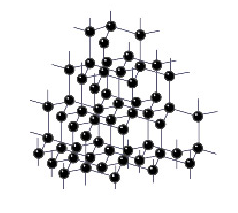
\includegraphics[scale=.32]{FQ/Termoquimica/diamante}};
\node (e) at (7,1) {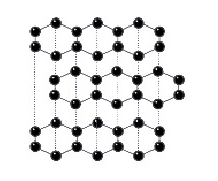
\includegraphics[scale=.32]{FQ/Termoquimica/grafite}};
\node at (n1) [red,font=\bfseries,below=.75cm] (f)  {forma + estável};
\end{tikzpicture}
\end{frame}



\begin{frame}[label={sec:org390612e}]{Oxigênio (O)}

\begin{tikzpicture}
% Axis y
\draw[->,ultra thick] (0,0)--(0,6) node[above]{$\Delta$H (\unit{\kilo\joule})};
% Axis X
\draw[-,ultra thick] (0,1)--(5,1) node[xshift=-2.3cm,anchor=south] (n1) {Oxigênio Atômico};
 \draw[-,ultra thick] (0,3)--(5,3) node[xshift=-2.3cm,anchor=south] (n2) {Ozônio};
\draw[-,ultra thick] (0,5)--(5,5) node[xshift=-2.3cm,anchor=south] (n3) {Oxigênio Molecular};
%\draw[->,ultra thick] (4,1)--(4,3.8);
 %\node[blue,font=\bfseries] (c) at (2,2.5) {$\enthalpy{1.9}$};
\node (d) at (8,1) {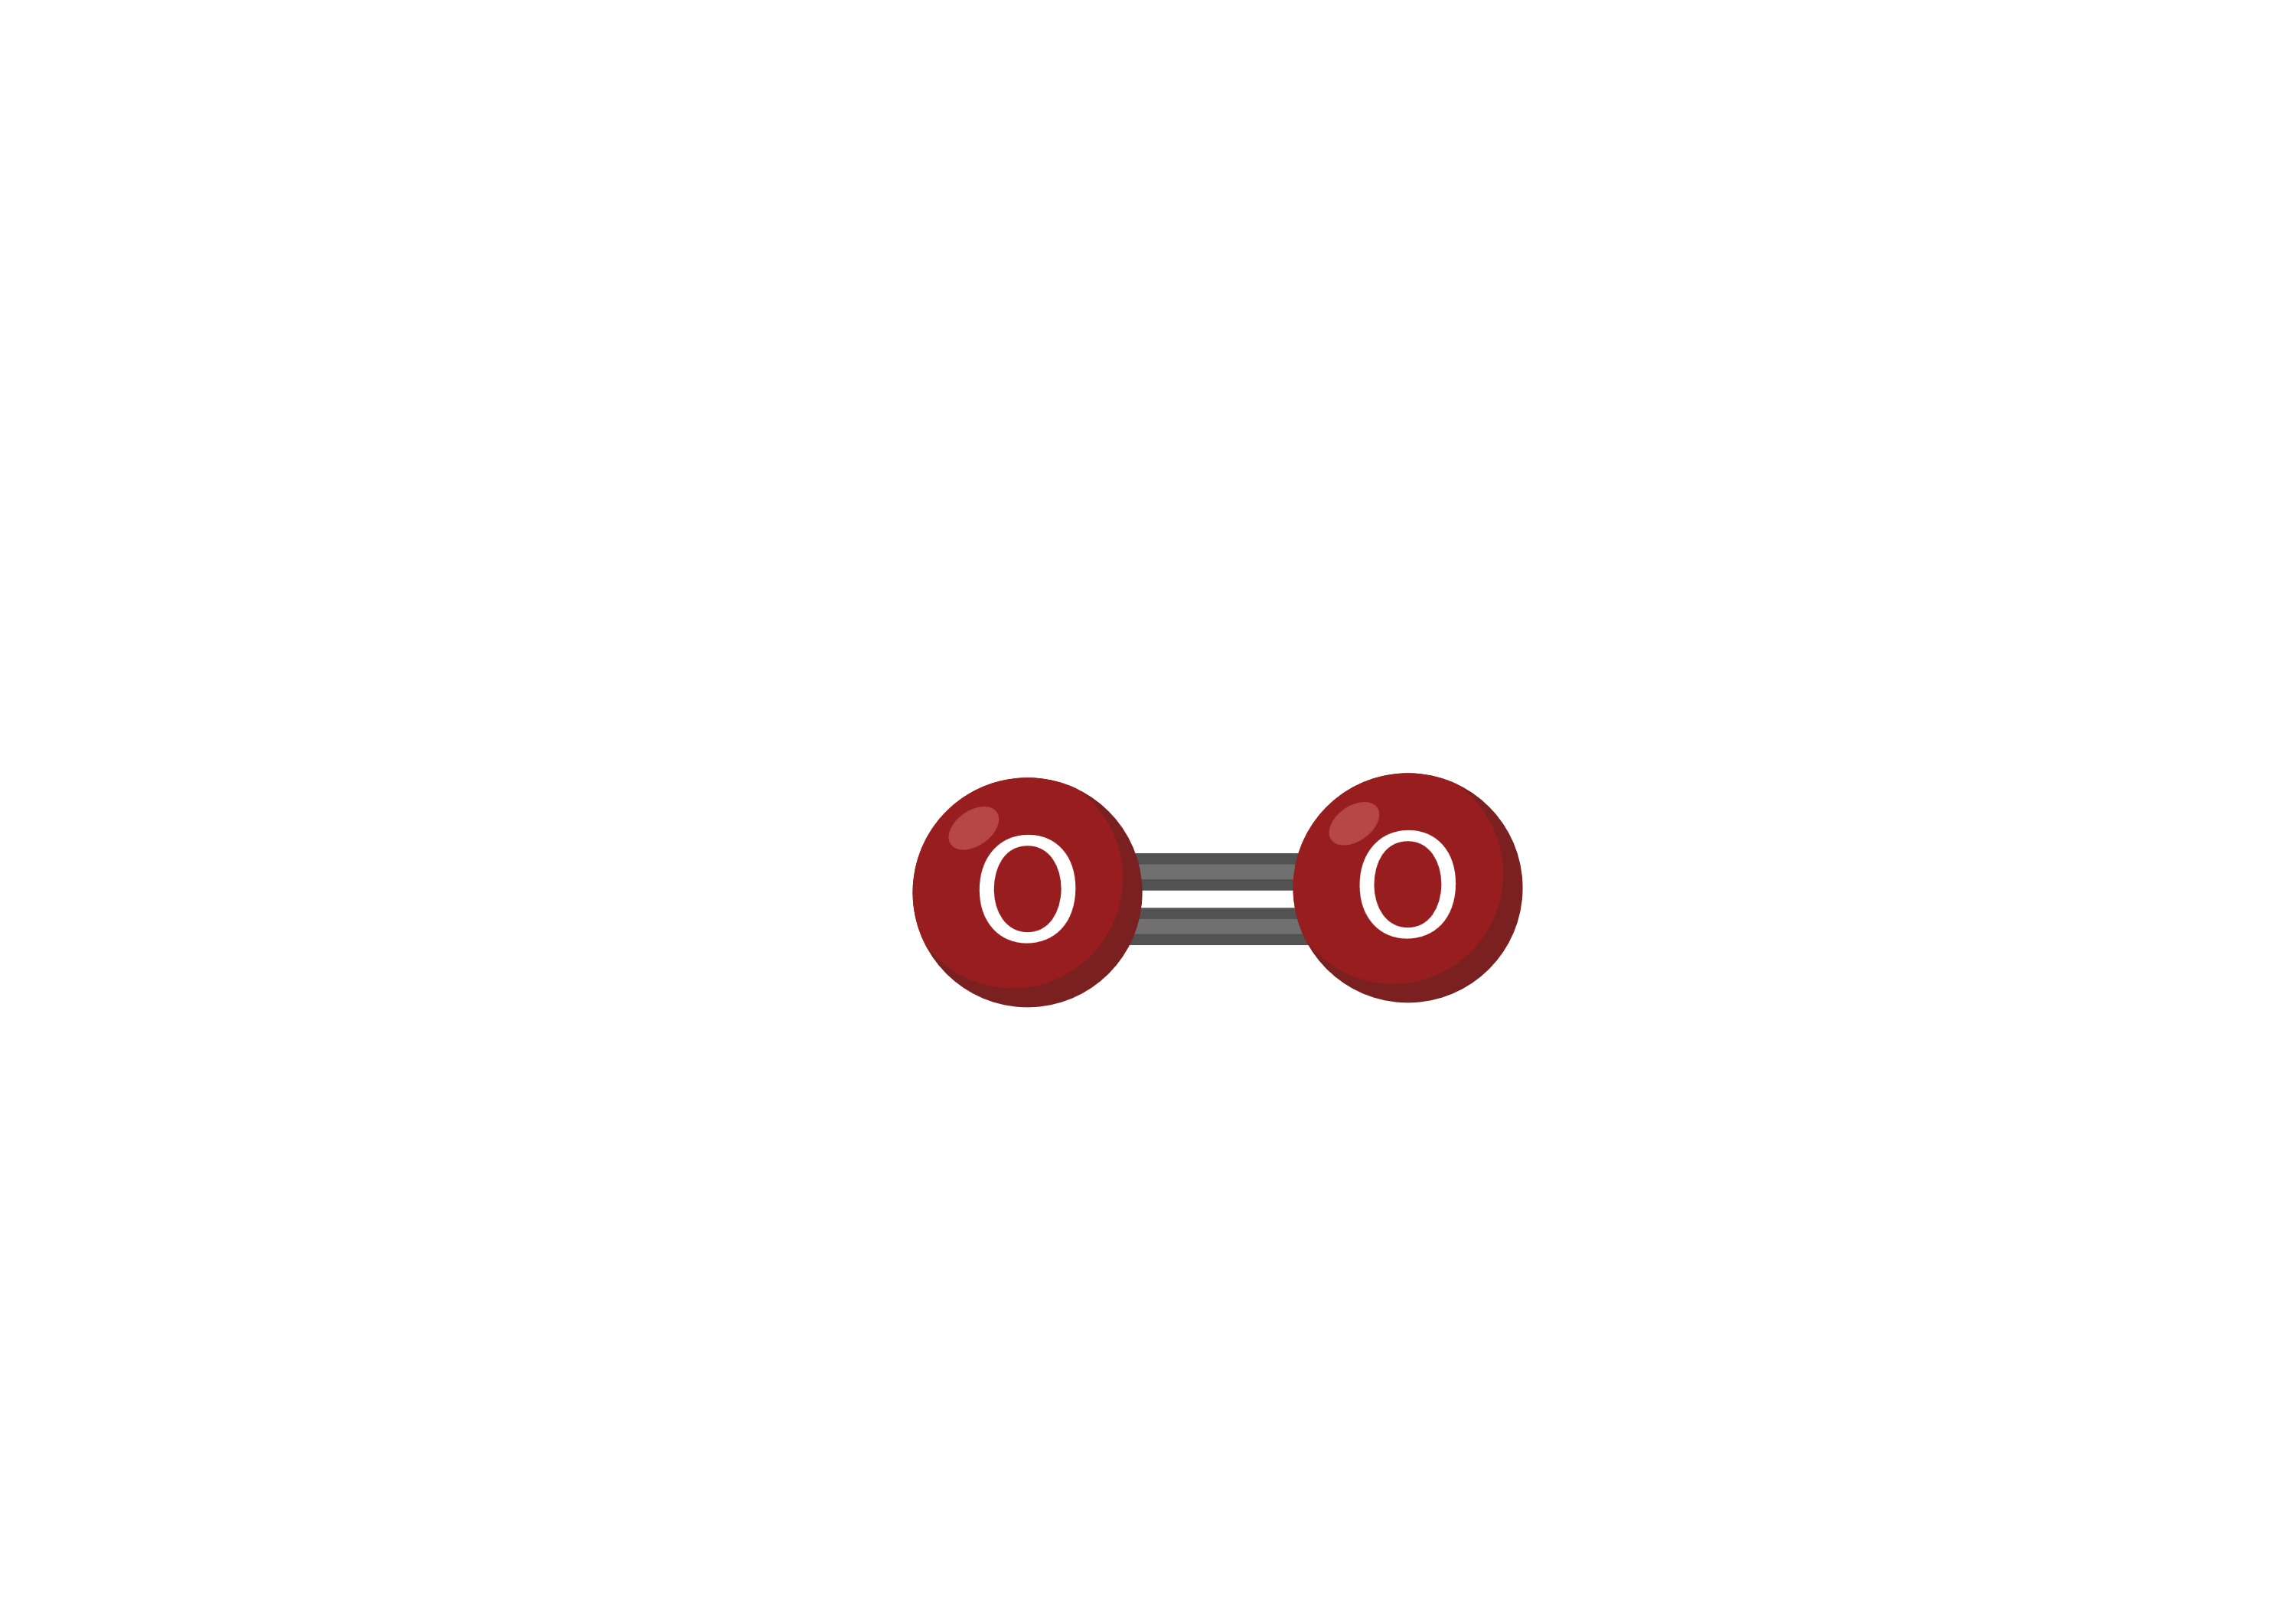
\includegraphics[scale=.3]{FQ/Termoquimica/Oxigen}};
\node (e) at (8,3.3) {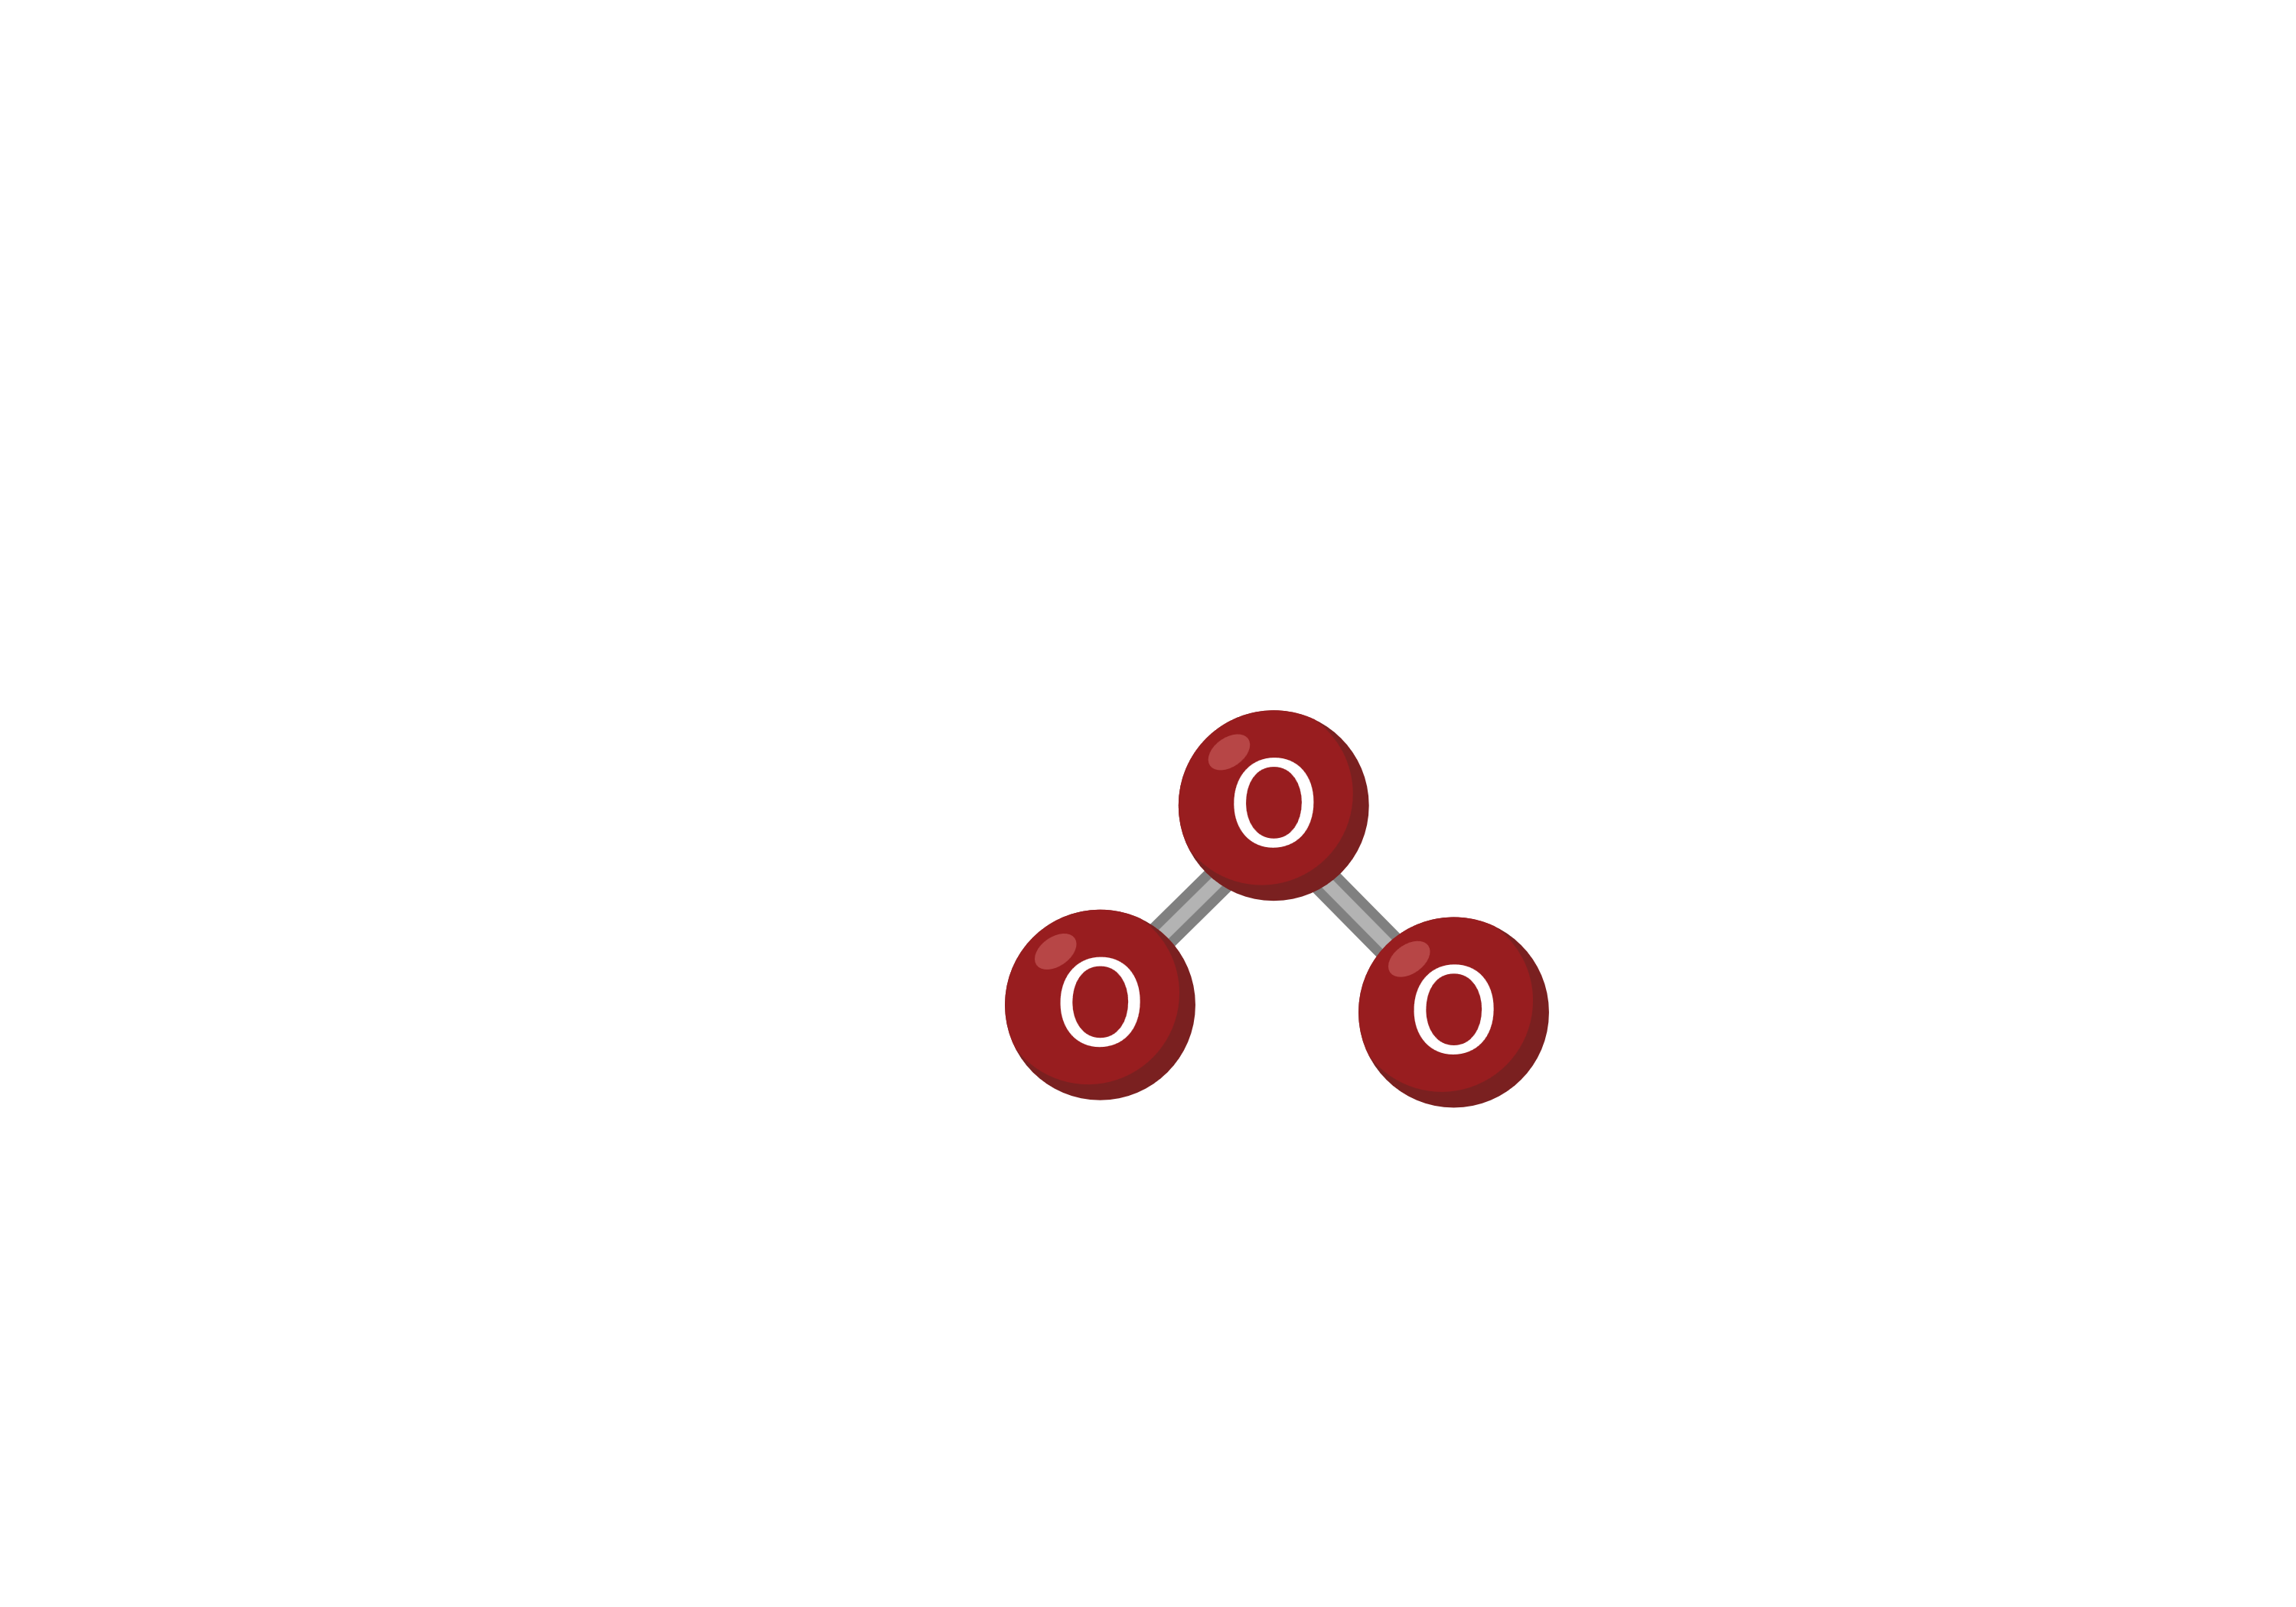
\includegraphics[scale=.3]{FQ/Termoquimica/Ozone}};
\node (f) at (8,5.2) {
\includegraphics[scale=.2]{FQ/Termoquimica/OxigenMolecular}};
\node at (n1) [red,font={\bfseries},below=.75cm] (g)  {forma + estável};
\node (text1) at (-.41,1) {0};
\node (text2) at (-0.46,3) {142,1};
\node (text3) at (-0.46,5) {249,1};
\end{tikzpicture}
\end{frame}




\begin{frame}[label={sec:org5dd99e6}]{Enxofre (S)}

\begin{tikzpicture}
% Axis y
\draw[->,ultra thick] (0,0)--(0,5) node[above]{$\Delta$H};
% Axis X
\draw[-,ultra thick] (0,1)--(5,1) node[xshift=-2.3cm,anchor=south] (n1) {S\textsubscript{monocíclico}};
 \draw[-,ultra thick] (0,4)--(5,4) node[xshift=-2.3cm,anchor=south] (n2) {S\textsubscript{rômbico}};
\draw[->,ultra thick] (4.5,1)--(4.5,3.8);
  \node[blue,font=\bfseries] (c) at (2,2.5) {$\enthalpy[unit=\kilo\cal\per\mol]{-4.3}$};
\node (d) at (7,4) {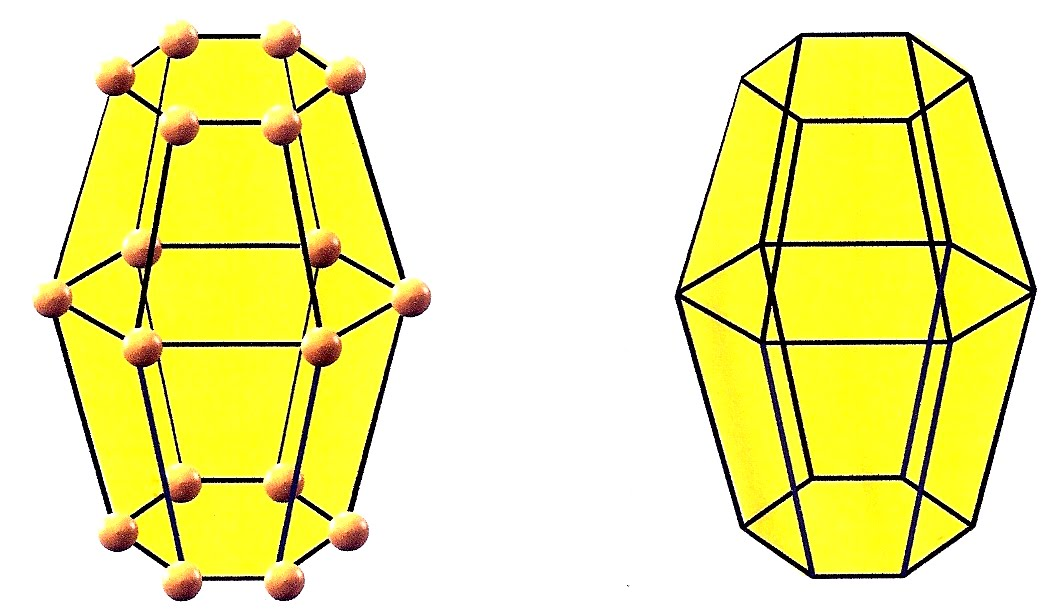
\includegraphics[scale=.09]{FQ/Termoquimica/EnxofreRom.jpg}};
\node (e) at (7,1) {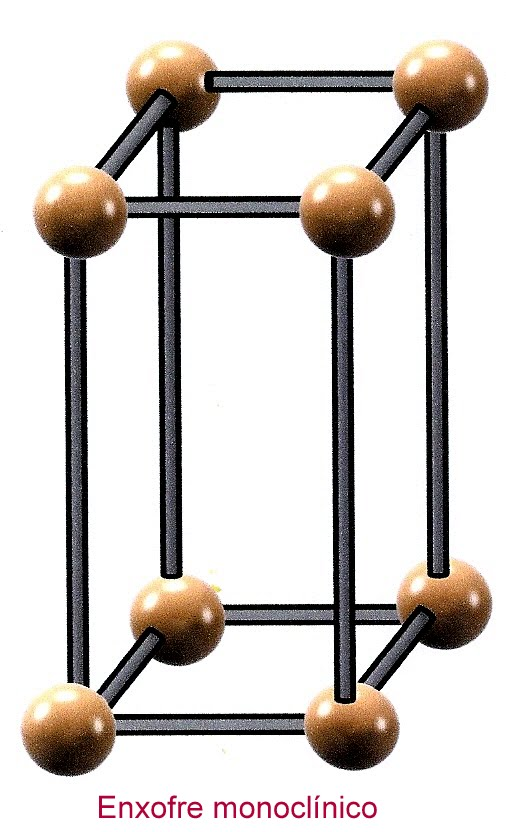
\includegraphics[scale=.09]{FQ/Termoquimica/EnxofreMono.jpg}};
%\node at (n1) [red,font=\bfseries,below=.75cm] (f)  {forma + estável};
\node at (d) [font=\small, above=1.2cm] (g) {S\textsubscript{romb.} + \ch{O2\gas{} -> SO2\gas{}} };
\node at (e) [font=\small, below=1.2cm] (h) {S\textsubscript{mono} + \ch{O2\gas{} -> SO2\gas{}} };
\end{tikzpicture}
\end{frame}



\begin{frame}[label={sec:orgefc5579}]{Fósforo (P)}
\begin{center}
\begin{tikzpicture}
\node (fig) at (0,0) {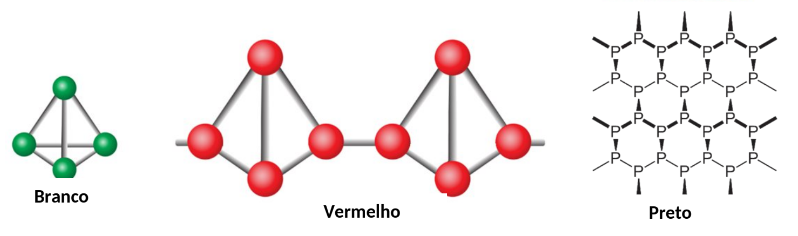
\includegraphics[scale=.5]{FQ/Termoquimica/Fosforo.png}};
\node[single arrow, draw=black, fill=red8!30, minimum width = 10pt, single arrow head extend=3pt, minimum height=10mm, below=1cm of fig,font=\bfseries] {Ordem descrescente de estabilidade}; % length of arrow
\end{tikzpicture}
\end{center}
\end{frame}




\section{Entalpia Padrão}
\label{sec:orge687fcf}

\begin{frame}[label={sec:org4344541}]{Entalpia padrão (\(\Delta\)Hº)}
\begin{itemize}
\item \alert{Entalpia de padrão (\(\Delta\)Hº )} devido à impossibilidade de determinarmos diretamente a entalpia das substâncias, trabalhamos com a variação de entalpia (\(\Delta\)H). Porém, a variação de entalpia de uma reação depende da temperatura, da pressão, do estado físico, do número de mols e da variedade alotrópica das substâncias envolvidas.
\item O estado padrão de uma substância corresponde à sua forma mais estável, a 1 atm, a 25 °C. A entalpia padrão de uma substância é indicada por \(\Delta\)H\(^0\).
\end{itemize}

Por convenção foi estabelecido que:

\begin{bclogo}[logo=\bcinfo]{Definição}
\emph{\alert{“Toda substância simples, no estado padrão e na sua forma alotrópica mais estável (mais comum), tem entalpia (H) igual a zero.”}}
\end{bclogo}
\end{frame}



\section{Entalpia de padrão de formação}
\label{sec:orgf76332b}

\begin{frame}[label={sec:org3a84a32}]{Entalpia Padrão de Formação}
\alert{Entalpia Padrão de Formação:} é a variação de entalpia que ocorre na formação de 1 mol de uma substância composta a partir de substâncias simples no estado padrão. 

\begin{bclogo}[logo=\bcinfo]{Exemplo \ch{H2O} (a \SI{25}{\celsius} e 1 atm)}
\small
\begin{reactions*}
H2_{\gas} + {1/2} O2_{\gas} -> H2O_{\lqdd} & $\qquad \enthalpy[unit=\kilo\cal\per\mole]{-68.4}$ \\ % \(\Delta\)H_f^0 = - 68,4 Kcal/mol
H2_{\gas} + {1/2} O2_{\gas} -> H2O_{\lqdd} & $\qquad \enthalpy[unit=\kilo\joule\per\mole]{-285}$ 
\end{reactions*}
\end{bclogo}


Observe que todos os reagentes são substâncias simples no estado padrão
\begin{reactions*}
H2\gas{} ->  H^0 = & \(\enthalpy{0}\)  \\
O2\gas{} ->  H^0 = & \(\enthalpy{0}\)
\end{reactions*}
\end{frame}



\begin{frame}[label={sec:org6c57730}]{Equação de Formação}
\begin{bclogo}[logo=\bcinfo]{Exemplo}
\begin{reactions*}
C\sld{} + O2\gas{} -> CO2\gas{} &  \\
H2\gas{} + 1/2 O2\gas{} -> H2O\lqdd{} & \\
\end{reactions*}
\end{bclogo}
\end{frame}


\section{Tipos de Entalpia}
\label{sec:org0b24c82}

\begin{frame}[label={sec:org5253d40}]{Entalpia de dissolução ( $\Delta$H$_{\mathrm{dissol.}}$ )}
O calor de dissolução é a variação de entalpia associada à dissolução de um mol de uma substância num determinado solvente para preparar uma solução diluída ideal:

\begin{bclogo}[logo=\bcinfo]{Exemplo (a \SI{25}{\celsius} e 1 atm)}
\begin{reactions*}
HC$\ell$\gas{} + H2O\lqdd{} -> HC$\ell$(aq)  & $\quad \enthalpy[unit=\kilo\cal\per\mol]{-18}$
\end{reactions*}
\end{bclogo}
\end{frame}


\begin{frame}[label={sec:orgb0f9f17}]{Entalpia de neutralização ( $\Delta$H$_{\mathrm{neutr.}}$ )}
\begin{itemize}
\item O calor de neutralização é a variação de entalpia associada à formação de 1 mol de  \ch{H2O\lqdd{}} a partir de 1 mol de  \ch{H^+_{\aq{}}} e 1 mol de  \ch{OH^-_{\aq{}}}, no estado padrão, em reações de neutralização entre ácidos e bases.
\end{itemize}

A entalpia de neutralização é praticamente constante no caso de ácidos e bases fortes.

\begin{bclogo}[logo=\bcinfo]{Exemplo}
\begin{reactions*}
HC$\ell$\aq{} + NaOH\aq{} -> NaC$\ell$\aq{} + H2O\lqdd{} &  $\qquad \enthalpy[unit=\kilo\cal]{-13.8}$ \\
HNO3\aq{} + KOH\aq{} -> KNO3\aq{} + H2O\lqdd{} & $\qquad \enthalpy[unit=\kilo\cal]{-13.8}$
\end{reactions*}
\end{bclogo}
Isto ocorre porque a reação que realmente acontece é:


\begin{reaction*}
H^+\aq{} + OH^-\aq{} ->  H2O\lqdd{}  $\qquad \enthalpy[unit=\kilo\cal]{-13.8}$
\end{reaction*}
\end{frame}


\begin{frame}[label={sec:org673a943}]{Cálculo de ΔH por entalpia de formação}
\begin{question}
\alert{(Fuvest)} A seguir são fornecidos dados relativos ao etanol hidratado e à gasolina.

\begin{talltblr}[
note{*} = {(U. M. = unidade monetária arbitrária.)},
caption ={Dados  relativos ao etanol hidratado e à gasolina.},
]
{
colspec = {cccc}, colsep = 3mm, hlines = {1pt, white},
row{1} = {2em,azure2,fg=white,font=\bfseries\sffamily},
}
Combustível &	{Calor de \\ Combustão (kcal/g)}  &	{Densidade \\ (kg/L)} &	{Preço por \\ litro (U. M.) \TblrNote{*}} \\
Etanol hidratado &	6,0  &	0,80  &	65 \\
Gasolina &	11,5 &	0,70 &	100 \\
\hline
\end{talltblr}


Calcule:
\begin{choice}
\choice As energias liberadas na combustão de 1 L de cada combustível.
\choice Os custos de 1 000 kcal (em U. M.) provenientes da queima do etanol e da gasolina.
\end{choice}
\end{question}
\end{frame}


\begin{frame}[label={sec:org14dd778}]{}
\begin{answer}[print=true]
Transforme as unidades equivalentes

a)

\alert{Etanol} = 0,80 kg/L = 800 g/L   \ch{->} 6 kcal/\cancel{g} $\times$ 800 \cancel{g}/L  = 4800 kcal/L 

\alert{Gasolina} = 0,70 kg/L = 700 g/L  \ch{->} 11,5 kcal/\cancel{g} $\times$ 700 \cancel{g}/L = 8050 kcal/L  

b)

\alert{Etanol}

\begin{align*}
& 65 ~\text{\small U.M.} -\!\!\!-\!\!\!- 4800~\text{\small kcal}\\
& x~\text{\small U.M.} -\!\!\!-\!\!\!- 1000~\text{\small kcal}
& x = 13,54 ~\text{U.M.}
\end{align*}

\alert{Gasolina} 

\begin{align*}
& 100 ~\text{\small U.M.} -\!\!\!-\!\!\!- 8050~\text{\small kcal}\\
& x~\text{\small U.M.} -\!\!\!-\!\!\!- 1000 ~\text{\small kcal}
& x = 12,42 ~\text{U.M.} 
\end{align*}
\end{answer}
\end{frame}



\begin{frame}[label={sec:org22690ae}]{}
\begin{question}
\small 
\alert{(UERJ)} O alumínio é utilizado como redutor de óxidos, no processo denominado de aluminotermia, conforme mostra a equação química:

\begin{reaction*}
8 A$\ell$\sld{} + 3 Mn3O4\sld{} -> 4 A$\ell$2O3\sld{} + 9 Mn\sld{}
\end{reaction*}


Observe a tabela:

\begin{center}
\begin{tblr}[
]{
colspec = {ccc}, colsep = 2mm, hlines = {1pt, white},
row{1} = {2em,azure2,fg=white,font=\bfseries},
}
Substância & Entalpia de Formação $\Delta$H a 298 K \\ %\hline
\ch{A$\ell$2O3\sld{}} & - 1667,8 \\
\ch{Mn3O2\sld{}} & - 1385,5 \\ \hline
\end{tblr}
\end{center}

Segundo a equação acima, para a obtenção do  \ch{Mn\sld{}}, a variação de entalpia, na temperatura de 298 K, em KJ, é de:

\begin{choice}(4)
\choice -282,5
\choice -2515,3
\choice -3053,1
\choice -10827,1
\end{choice}
\end{question}
\end{frame}


\begin{frame}[label={sec:org68dd2f0}]{}
\begin{answer}[print=true]
\scriptsize
\alert{Letra b)}. Veja o passo a passo para a determinação da variação de entalpia:

\begin{description}
\item[{1º Passo:}] O cálculo da entalpia dos produtos (H\textsubscript{p}) é feito pela multiplicação do coeficiente de cada participante pela sua entalpia e, depois, pela soma dos resultados.
\item[{2º Passo:}] O cálculo da entalpia dos reagentes (H\textsubscript{r}) é feito pela multiplicação do coeficiente de cada participante pela sua entalpia e, depois, pela soma dos resultados.
\end{description}


\begin{tblr}[
]{
 			colspec = {lcc}, colsep = 1mm, hlines = {2pt, white},
% 			row{1,3} = {2em,azure3,fg=white,font=\bfseries\sffamily},
}
$\Delta$ H = & H\textsubscript{produtos} &  \hspace{1.5cm}  -  H\textsubscript{reagentes} \\
$\Delta$ H = & [ ( 4 $\cdot$ $\Delta$ H\textsubscript{\ch{A$\ell$2O3\sld{}}} + 9 $\cdot$ $\Delta$ H\textsubscript{\ch{Mn\sld{}}}) ]  & -   [ 8  $\cdot$ $\Delta$ H\textsubscript{\ch{A$\ell$\sld{}}} + 3 $\cdot$ $\Delta$ H\textsubscript{\ch{Mn3O4\sld{}}}]\\
$\Delta$ H= & [4 \cdot (-1667,8) + 9 \cdot (0)]   & -  [8 \cdot (0) + 3 \cdot (-1385,3)]\\
$\Delta$ H= & [- 6671,2]  & -   [- 4155,9]\\
$\Delta$ H = & \hspace{2.0cm}    -2515,3 ~\unit{\kilo\joule\per\mol}&&
\end{tblr}
\end{answer}
\end{frame}

\begin{frame}[label={sec:org9188dfe}]{Fim da Aula}
\begin{tikzpicture}
\node[graduate,sword, minimum size=1cm]{ \bfseries Bons Estudos !!!!};
\end{tikzpicture}
\begin{center}
\begin{tblr}
{ccc}
Download Aula & & Lista de Exercícios \\
 \qrcode[height=2in]{https://mark.nl.tab.digital/s/8ocJrDKNYRkxmfG} & & \qrcode[height=2in]{https://mark.nl.tab.digital/s/LQwiRJGiybMj32g}\\
 \end{tblr}
 \end{center}
\end{frame}
\end{document}
